\documentclass[1p]{elsarticle_modified}
%\bibliographystyle{elsarticle-num}

%\usepackage[colorlinks]{hyperref}
%\usepackage{abbrmath_seonhwa} %\Abb, \Ascr, \Acal ,\Abf, \Afrak
\usepackage{amsfonts}
\usepackage{amssymb}
\usepackage{amsmath}
\usepackage{amsthm}
\usepackage{scalefnt}
\usepackage{amsbsy}
\usepackage{kotex}
\usepackage{caption}
\usepackage{subfig}
\usepackage{color}
\usepackage{graphicx}
\usepackage{xcolor} %% white, black, red, green, blue, cyan, magenta, yellow
\usepackage{float}
\usepackage{setspace}
\usepackage{hyperref}

\usepackage{tikz}
\usetikzlibrary{arrows}

\usepackage{multirow}
\usepackage{array} % fixed length table
\usepackage{hhline}

%%%%%%%%%%%%%%%%%%%%%
\makeatletter
\renewcommand*\env@matrix[1][\arraystretch]{%
	\edef\arraystretch{#1}%
	\hskip -\arraycolsep
	\let\@ifnextchar\new@ifnextchar
	\array{*\c@MaxMatrixCols c}}
\makeatother %https://tex.stackexchange.com/questions/14071/how-can-i-increase-the-line-spacing-in-a-matrix
%%%%%%%%%%%%%%%

\usepackage[normalem]{ulem}

\newcommand{\msout}[1]{\ifmmode\text{\sout{\ensuremath{#1}}}\else\sout{#1}\fi}
%SOURCE: \msout is \stkout macro in https://tex.stackexchange.com/questions/20609/strikeout-in-math-mode

\newcommand{\cancel}[1]{
	\ifmmode
	{\color{red}\msout{#1}}
	\else
	{\color{red}\sout{#1}}
	\fi
}

\newcommand{\add}[1]{
	{\color{blue}\uwave{#1}}
}

\newcommand{\replace}[2]{
	\ifmmode
	{\color{red}\msout{#1}}{\color{blue}\uwave{#2}}
	\else
	{\color{red}\sout{#1}}{\color{blue}\uwave{#2}}
	\fi
}

\newcommand{\Sol}{\mathcal{S}} %segment
\newcommand{\D}{D} %diagram
\newcommand{\A}{\mathcal{A}} %arc


%%%%%%%%%%%%%%%%%%%%%%%%%%%%%5 test

\def\sl{\operatorname{\textup{SL}}(2,\Cbb)}
\def\psl{\operatorname{\textup{PSL}}(2,\Cbb)}
\def\quan{\mkern 1mu \triangleright \mkern 1mu}

\theoremstyle{definition}
\newtheorem{thm}{Theorem}[section]
\newtheorem{prop}[thm]{Proposition}
\newtheorem{lem}[thm]{Lemma}
\newtheorem{ques}[thm]{Question}
\newtheorem{cor}[thm]{Corollary}
\newtheorem{defn}[thm]{Definition}
\newtheorem{exam}[thm]{Example}
\newtheorem{rmk}[thm]{Remark}
\newtheorem{alg}[thm]{Algorithm}

\newcommand{\I}{\sqrt{-1}}
\begin{document}

%\begin{frontmatter}
%
%\title{Boundary parabolic representations of knots up to 8 crossings}
%
%%% Group authors per affiliation:
%\author{Yunhi Cho} 
%\address{Department of Mathematics, University of Seoul, Seoul, Korea}
%\ead{yhcho@uos.ac.kr}
%
%
%\author{Seonhwa Kim} %\fnref{s_kim}}
%\address{Center for Geometry and Physics, Institute for Basic Science, Pohang, 37673, Korea}
%\ead{ryeona17@ibs.re.kr}
%
%\author{Hyuk Kim}
%\address{Department of Mathematical Sciences, Seoul National University, Seoul 08826, Korea}
%\ead{hyukkim@snu.ac.kr}
%
%\author{Seokbeom Yoon}
%\address{Department of Mathematical Sciences, Seoul National University, Seoul, 08826,  Korea}
%\ead{sbyoon15@snu.ac.kr}
%
%\begin{abstract}
%We find all boundary parabolic representation of knots up to 8 crossings.
%
%\end{abstract}
%\begin{keyword}
%    \MSC[2010] 57M25 
%\end{keyword}
%
%\end{frontmatter}

%\linenumbers
%\tableofcontents
%
\newcommand\colored[1]{\textcolor{white}{\rule[-0.35ex]{0.8em}{1.4ex}}\kern-0.8em\color{red} #1}%
%\newcommand\colored[1]{\textcolor{white}{ #1}\kern-2.17ex	\textcolor{white}{ #1}\kern-1.81ex	\textcolor{white}{ #1}\kern-2.15ex\color{red}#1	}

{\Large $\underline{12a_{1023}~(K12a_{1023})}$}

\setlength{\tabcolsep}{10pt}
\renewcommand{\arraystretch}{1.6}
\vspace{1cm}\begin{tabular}{m{100pt}>{\centering\arraybackslash}m{274pt}}
\multirow{5}{120pt}{
	\centering
	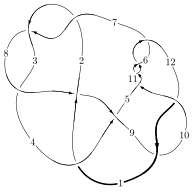
\includegraphics[width=112pt]{../../../GIT/diagram.site/Diagrams/png/1824_12a_1023.png}\\
\ \ \ A knot diagram\footnotemark}&
\allowdisplaybreaks
\textbf{Linearized knot diagam} \\
\cline{2-2}
 &
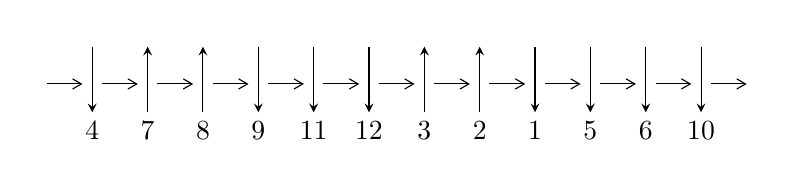
\begin{tikzpicture}[x=20pt, y=17pt]
	% nodes
	\node (C0) at (0, 0) {};
	\node (C1) at (1, 0) {};
	\node (C1U) at (1, +1) {};
	\node (C1D) at (1, -1) {4};

	\node (C2) at (2, 0) {};
	\node (C2U) at (2, +1) {};
	\node (C2D) at (2, -1) {7};

	\node (C3) at (3, 0) {};
	\node (C3U) at (3, +1) {};
	\node (C3D) at (3, -1) {8};

	\node (C4) at (4, 0) {};
	\node (C4U) at (4, +1) {};
	\node (C4D) at (4, -1) {9};

	\node (C5) at (5, 0) {};
	\node (C5U) at (5, +1) {};
	\node (C5D) at (5, -1) {11};

	\node (C6) at (6, 0) {};
	\node (C6U) at (6, +1) {};
	\node (C6D) at (6, -1) {12};

	\node (C7) at (7, 0) {};
	\node (C7U) at (7, +1) {};
	\node (C7D) at (7, -1) {3};

	\node (C8) at (8, 0) {};
	\node (C8U) at (8, +1) {};
	\node (C8D) at (8, -1) {2};

	\node (C9) at (9, 0) {};
	\node (C9U) at (9, +1) {};
	\node (C9D) at (9, -1) {1};

	\node (C10) at (10, 0) {};
	\node (C10U) at (10, +1) {};
	\node (C10D) at (10, -1) {5};

	\node (C11) at (11, 0) {};
	\node (C11U) at (11, +1) {};
	\node (C11D) at (11, -1) {6};

	\node (C12) at (12, 0) {};
	\node (C12U) at (12, +1) {};
	\node (C12D) at (12, -1) {10};
	\node (C13) at (13, 0) {};

	% arrows
	\draw[->,>={angle 60}]
	(C0) edge (C1) (C1) edge (C2) (C2) edge (C3) (C3) edge (C4) (C4) edge (C5) (C5) edge (C6) (C6) edge (C7) (C7) edge (C8) (C8) edge (C9) (C9) edge (C10) (C10) edge (C11) (C11) edge (C12) (C12) edge (C13) ;	\draw[->,>=stealth]
	(C1U) edge (C1D) (C2D) edge (C2U) (C3D) edge (C3U) (C4U) edge (C4D) (C5U) edge (C5D) (C6U) edge (C6D) (C7D) edge (C7U) (C8D) edge (C8U) (C9U) edge (C9D) (C10U) edge (C10D) (C11U) edge (C11D) (C12U) edge (C12D) ;
	\end{tikzpicture} \\
\hhline{~~} \\& 
\textbf{Solving Sequence} \\ \cline{2-2} 
 &
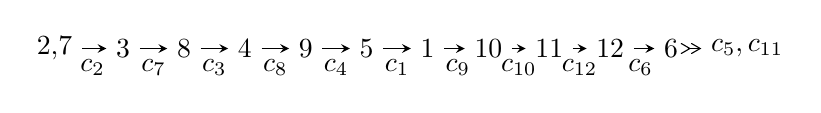
\begin{tikzpicture}[x=22pt, y=7pt]
	% node
	\node (A0) at (-1/8, 0) {2,7};
	\node (A1) at (1, 0) {3};
	\node (A2) at (2, 0) {8};
	\node (A3) at (3, 0) {4};
	\node (A4) at (4, 0) {9};
	\node (A5) at (5, 0) {5};
	\node (A6) at (6, 0) {1};
	\node (A7) at (7, 0) {10};
	\node (A8) at (8, 0) {11};
	\node (A9) at (9, 0) {12};
	\node (A10) at (10, 0) {6};
	\node (C1) at (1/2, -1) {$c_{2}$};
	\node (C2) at (3/2, -1) {$c_{7}$};
	\node (C3) at (5/2, -1) {$c_{3}$};
	\node (C4) at (7/2, -1) {$c_{8}$};
	\node (C5) at (9/2, -1) {$c_{4}$};
	\node (C6) at (11/2, -1) {$c_{1}$};
	\node (C7) at (13/2, -1) {$c_{9}$};
	\node (C8) at (15/2, -1) {$c_{10}$};
	\node (C9) at (17/2, -1) {$c_{12}$};
	\node (C10) at (19/2, -1) {$c_{6}$};
	\node (A11) at (45/4, 0) {$c_{5},c_{11}$};

	% edge
	\draw[->,>=stealth]	
	(A0) edge (A1) (A1) edge (A2) (A2) edge (A3) (A3) edge (A4) (A4) edge (A5) (A5) edge (A6) (A6) edge (A7) (A7) edge (A8) (A8) edge (A9) (A9) edge (A10) ;
	\draw[->>,>={angle 60}]	
	(A10) edge (A11);
\end{tikzpicture} \\ 

\end{tabular} \\

\footnotetext{
The image of knot diagram is generated by the software ``\textbf{Draw programme}" developed by Andrew Bartholomew(\url{http://www.layer8.co.uk/maths/draw/index.htm\#Running-draw}), where we modified some parts for our purpose(\url{https://github.com/CATsTAILs/LinksPainter}).
}\phantom \\ \newline 
\centering \textbf{Ideals for irreducible components\footnotemark of $X_{\text{par}}$} 
 
\begin{align*}
I^u_{1}&=\langle 
u^{63}- u^{62}+\cdots+4 u^3-1\rangle \\
\\
\end{align*}
\raggedright * 1 irreducible components of $\dim_{\mathbb{C}}=0$, with total 63 representations.\\
\footnotetext{All coefficients of polynomials are rational numbers. But the coefficients are sometimes approximated in decimal forms when there is not enough margin.}
\newpage
\renewcommand{\arraystretch}{1}
\centering \section*{I. $I^u_{1}= \langle u^{63}- u^{62}+\cdots+4 u^3-1 \rangle$}
\flushleft \textbf{(i) Arc colorings}\\
\begin{tabular}{m{7pt} m{180pt} m{7pt} m{180pt} }
\flushright $a_{2}=$&$\begin{pmatrix}1\\0\end{pmatrix}$ \\
\flushright $a_{7}=$&$\begin{pmatrix}0\\u\end{pmatrix}$ \\
\flushright $a_{3}=$&$\begin{pmatrix}1\\- u^2\end{pmatrix}$ \\
\flushright $a_{8}=$&$\begin{pmatrix}u\\- u^3+u\end{pmatrix}$ \\
\flushright $a_{4}=$&$\begin{pmatrix}- u^2+1\\u^4-2 u^2\end{pmatrix}$ \\
\flushright $a_{9}=$&$\begin{pmatrix}- u^3+2 u\\- u^3+u\end{pmatrix}$ \\
\flushright $a_{5}=$&$\begin{pmatrix}- u^{10}+5 u^8-8 u^6+3 u^4+u^2+1\\- u^{10}+4 u^8-5 u^6+2 u^4- u^2\end{pmatrix}$ \\
\flushright $a_{1}=$&$\begin{pmatrix}u^6-3 u^4+2 u^2+1\\- u^8+4 u^6-4 u^4\end{pmatrix}$ \\
\flushright $a_{10}=$&$\begin{pmatrix}u^{17}-8 u^{15}+25 u^{13}-36 u^{11}+19 u^9+4 u^7-2 u^5-4 u^3+u\\- u^{19}+9 u^{17}-32 u^{15}+55 u^{13}-43 u^{11}+9 u^9+4 u^5- u^3+u\end{pmatrix}$ \\
\flushright $a_{11}=$&$\begin{pmatrix}u^{39}-18 u^{37}+\cdots-6 u^5-6 u^3\\u^{39}-17 u^{37}+\cdots+3 u^5+u\end{pmatrix}$ \\
\flushright $a_{12}=$&$\begin{pmatrix}u^{28}-13 u^{26}+\cdots+u^2+1\\- u^{30}+14 u^{28}+\cdots-4 u^4- u^2\end{pmatrix}$ \\
\flushright $a_{6}=$&$\begin{pmatrix}u^{57}-26 u^{55}+\cdots+2 u^3+u\\- u^{59}+27 u^{57}+\cdots- u^3+u\end{pmatrix}$\\&\end{tabular}
\flushleft \textbf{(ii) Obstruction class $= -1$}\\~\\
\flushleft \textbf{(iii) Cusp Shapes $= 4 u^{61}-112 u^{59}+\cdots+4 u-2$}\\~\\
\newpage\renewcommand{\arraystretch}{1}
\flushleft \textbf{(iv) u-Polynomials at the component}\newline \\
\begin{tabular}{m{50pt}|m{274pt}}
Crossings & \hspace{64pt}u-Polynomials at each crossing \\
\hline $$\begin{aligned}c_{1}\end{aligned}$$&$\begin{aligned}
&u^{63}-13 u^{62}+\cdots+5048 u-367
\end{aligned}$\\
\hline $$\begin{aligned}c_{2},c_{3},c_{7}\end{aligned}$$&$\begin{aligned}
&u^{63}+u^{62}+\cdots+4 u^3+1
\end{aligned}$\\
\hline $$\begin{aligned}c_{4}\end{aligned}$$&$\begin{aligned}
&u^{63}- u^{62}+\cdots-16 u+1
\end{aligned}$\\
\hline $$\begin{aligned}c_{5},c_{6},c_{10}\\c_{11}\end{aligned}$$&$\begin{aligned}
&u^{63}+u^{62}+\cdots-2 u^4+1
\end{aligned}$\\
\hline $$\begin{aligned}c_{8}\end{aligned}$$&$\begin{aligned}
&u^{63}-3 u^{62}+\cdots-14 u+1
\end{aligned}$\\
\hline $$\begin{aligned}c_{9},c_{12}\end{aligned}$$&$\begin{aligned}
&u^{63}-11 u^{62}+\cdots+1032 u-113
\end{aligned}$\\
\hline
\end{tabular}\\~\\
\newpage\renewcommand{\arraystretch}{1}
\flushleft \textbf{(v) Riley Polynomials at the component}\newline \\
\begin{tabular}{m{50pt}|m{274pt}}
Crossings & \hspace{64pt}Riley Polynomials at each crossing \\
\hline $$\begin{aligned}c_{1}\end{aligned}$$&$\begin{aligned}
&y^{63}+23 y^{62}+\cdots+185728 y-134689
\end{aligned}$\\
\hline $$\begin{aligned}c_{2},c_{3},c_{7}\end{aligned}$$&$\begin{aligned}
&y^{63}-57 y^{62}+\cdots+12 y^2-1
\end{aligned}$\\
\hline $$\begin{aligned}c_{4}\end{aligned}$$&$\begin{aligned}
&y^{63}- y^{62}+\cdots-64 y-1
\end{aligned}$\\
\hline $$\begin{aligned}c_{5},c_{6},c_{10}\\c_{11}\end{aligned}$$&$\begin{aligned}
&y^{63}-69 y^{62}+\cdots+4 y^2-1
\end{aligned}$\\
\hline $$\begin{aligned}c_{8}\end{aligned}$$&$\begin{aligned}
&y^{63}-5 y^{62}+\cdots+96 y-1
\end{aligned}$\\
\hline $$\begin{aligned}c_{9},c_{12}\end{aligned}$$&$\begin{aligned}
&y^{63}+39 y^{62}+\cdots-28816 y-12769
\end{aligned}$\\
\hline
\end{tabular}\\~\\
\newpage\flushleft \textbf{(vi) Complex Volumes and Cusp Shapes}
$$\begin{array}{c|c|c}  
\text{Solutions to }I^u_{1}& \I (\text{vol} + \sqrt{-1}CS) & \text{Cusp shape}\\
 \hline 
\begin{aligned}
u &= \phantom{-}1.05857\phantom{ +0.000000I}\end{aligned}
 & -0.871869\phantom{ +0.000000I} & -9.57900\phantom{ +0.000000I} \\ \hline\begin{aligned}
u &= -1.124880 + 0.212975 I\end{aligned}
 & -4.94868 - 6.91271 I & \phantom{-0.000000 } 0 \\ \hline\begin{aligned}
u &= -1.124880 - 0.212975 I\end{aligned}
 & -4.94868 + 6.91271 I & \phantom{-0.000000 } 0 \\ \hline\begin{aligned}
u &= \phantom{-}1.148860 + 0.182186 I\end{aligned}
 & \phantom{-}2.18519 + 4.53135 I & \phantom{-0.000000 } 0 \\ \hline\begin{aligned}
u &= \phantom{-}1.148860 - 0.182186 I\end{aligned}
 & \phantom{-}2.18519 - 4.53135 I & \phantom{-0.000000 } 0 \\ \hline\begin{aligned}
u &= -0.830553 + 0.042703 I\end{aligned}
 & -8.69415 + 0.00048 I & -9.30642 + 0.15839 I \\ \hline\begin{aligned}
u &= -0.830553 - 0.042703 I\end{aligned}
 & -8.69415 - 0.00048 I & -9.30642 - 0.15839 I \\ \hline\begin{aligned}
u &= -1.190630 + 0.128855 I\end{aligned}
 & \phantom{-}2.84482 - 1.03901 I & \phantom{-0.000000 } 0 \\ \hline\begin{aligned}
u &= -1.190630 - 0.128855 I\end{aligned}
 & \phantom{-}2.84482 + 1.03901 I & \phantom{-0.000000 } 0 \\ \hline\begin{aligned}
u &= -0.307202 + 0.707160 I\end{aligned}
 & -5.43312 - 10.27260 I & -7.72829 + 7.96510 I \\ \hline\begin{aligned}
u &= -0.307202 - 0.707160 I\end{aligned}
 & -5.43312 + 10.27260 I & -7.72829 - 7.96510 I \\ \hline\begin{aligned}
u &= \phantom{-}0.311428 + 0.693681 I\end{aligned}
 & \phantom{-}1.68556 + 7.55058 I & -4.18504 - 9.18442 I \\ \hline\begin{aligned}
u &= \phantom{-}0.311428 - 0.693681 I\end{aligned}
 & \phantom{-}1.68556 - 7.55058 I & -4.18504 + 9.18442 I \\ \hline\begin{aligned}
u &= -0.317156 + 0.675863 I\end{aligned}
 & \phantom{-}2.25968 - 3.54520 I & -2.30097 + 2.95262 I \\ \hline\begin{aligned}
u &= -0.317156 - 0.675863 I\end{aligned}
 & \phantom{-}2.25968 + 3.54520 I & -2.30097 - 2.95262 I \\ \hline\begin{aligned}
u &= -0.615511 + 0.402928 I\end{aligned}
 & -4.21282 + 6.36699 I & -5.11968 - 2.58502 I \\ \hline\begin{aligned}
u &= -0.615511 - 0.402928 I\end{aligned}
 & -4.21282 - 6.36699 I & -5.11968 + 2.58502 I \\ \hline\begin{aligned}
u &= \phantom{-}0.336084 + 0.649282 I\end{aligned}
 & -3.64458 + 1.06314 I & -5.63466 - 3.13287 I \\ \hline\begin{aligned}
u &= \phantom{-}0.336084 - 0.649282 I\end{aligned}
 & -3.64458 - 1.06314 I & -5.63466 + 3.13287 I \\ \hline\begin{aligned}
u &= -0.218313 + 0.688956 I\end{aligned}
 & -10.70060 - 3.40629 I & -12.54413 + 4.55404 I \\ \hline\begin{aligned}
u &= -0.218313 - 0.688956 I\end{aligned}
 & -10.70060 + 3.40629 I & -12.54413 - 4.55404 I \\ \hline\begin{aligned}
u &= \phantom{-}0.577950 + 0.406867 I\end{aligned}
 & \phantom{-}2.80271 - 3.72383 I & -1.35159 + 3.56435 I \\ \hline\begin{aligned}
u &= \phantom{-}0.577950 - 0.406867 I\end{aligned}
 & \phantom{-}2.80271 + 3.72383 I & -1.35159 - 3.56435 I \\ \hline\begin{aligned}
u &= \phantom{-}0.229540 + 0.647261 I\end{aligned}
 & -2.84257 + 2.89752 I & -11.56820 - 6.31602 I \\ \hline\begin{aligned}
u &= \phantom{-}0.229540 - 0.647261 I\end{aligned}
 & -2.84257 - 2.89752 I & -11.56820 + 6.31602 I \\ \hline\begin{aligned}
u &= \phantom{-}0.495663 + 0.468066 I\end{aligned}
 & -2.93186 + 2.65024 I & -3.65682 - 3.70204 I \\ \hline\begin{aligned}
u &= \phantom{-}0.495663 - 0.468066 I\end{aligned}
 & -2.93186 - 2.65024 I & -3.65682 + 3.70204 I \\ \hline\begin{aligned}
u &= -0.533777 + 0.423287 I\end{aligned}
 & \phantom{-}3.22952 - 0.19502 I & \phantom{-}0.24983 + 3.49872 I \\ \hline\begin{aligned}
u &= -0.533777 - 0.423287 I\end{aligned}
 & \phantom{-}3.22952 + 0.19502 I & \phantom{-}0.24983 - 3.49872 I \\ \hline\begin{aligned}
u &= \phantom{-}1.303640 + 0.225472 I\end{aligned}
 & -3.76308 - 0.34360 I & \phantom{-0.000000 } 0\\
 \hline 
 \end{array}$$\newpage$$\begin{array}{c|c|c}  
\text{Solutions to }I^u_{1}& \I (\text{vol} + \sqrt{-1}CS) & \text{Cusp shape}\\
 \hline 
\begin{aligned}
u &= \phantom{-}1.303640 - 0.225472 I\end{aligned}
 & -3.76308 + 0.34360 I & \phantom{-0.000000 } 0 \\ \hline\begin{aligned}
u &= -0.083521 + 0.671063 I\end{aligned}
 & -8.05532 + 3.57894 I & -11.69365 - 1.74226 I \\ \hline\begin{aligned}
u &= -0.083521 - 0.671063 I\end{aligned}
 & -8.05532 - 3.57894 I & -11.69365 + 1.74226 I \\ \hline\begin{aligned}
u &= \phantom{-}1.32555\phantom{ +0.000000I}\end{aligned}
 & -2.93780\phantom{ +0.000000I} & \phantom{-0.000000 } 0 \\ \hline\begin{aligned}
u &= -1.350050 + 0.193271 I\end{aligned}
 & \phantom{-}3.40243 - 1.30144 I & \phantom{-0.000000 } 0 \\ \hline\begin{aligned}
u &= -1.350050 - 0.193271 I\end{aligned}
 & \phantom{-}3.40243 + 1.30144 I & \phantom{-0.000000 } 0 \\ \hline\begin{aligned}
u &= \phantom{-}0.070290 + 0.619087 I\end{aligned}
 & -1.00852 - 1.48110 I & -8.78123 + 3.67726 I \\ \hline\begin{aligned}
u &= \phantom{-}0.070290 - 0.619087 I\end{aligned}
 & -1.00852 + 1.48110 I & -8.78123 - 3.67726 I \\ \hline\begin{aligned}
u &= \phantom{-}1.389370 + 0.217872 I\end{aligned}
 & \phantom{-}4.99399 + 3.97068 I & \phantom{-0.000000 } 0 \\ \hline\begin{aligned}
u &= \phantom{-}1.389370 - 0.217872 I\end{aligned}
 & \phantom{-}4.99399 - 3.97068 I & \phantom{-0.000000 } 0 \\ \hline\begin{aligned}
u &= \phantom{-}1.382970 + 0.269752 I\end{aligned}
 & -5.61347 + 6.88488 I & \phantom{-0.000000 } 0 \\ \hline\begin{aligned}
u &= \phantom{-}1.382970 - 0.269752 I\end{aligned}
 & -5.61347 - 6.88488 I & \phantom{-0.000000 } 0 \\ \hline\begin{aligned}
u &= -1.389830 + 0.251114 I\end{aligned}
 & \phantom{-}2.31904 - 6.16933 I & \phantom{-0.000000 } 0 \\ \hline\begin{aligned}
u &= -1.389830 - 0.251114 I\end{aligned}
 & \phantom{-}2.31904 + 6.16933 I & \phantom{-0.000000 } 0 \\ \hline\begin{aligned}
u &= -0.214690 + 0.530628 I\end{aligned}
 & -0.156297 - 1.165440 I & -2.55431 + 5.45798 I \\ \hline\begin{aligned}
u &= -0.214690 - 0.530628 I\end{aligned}
 & -0.156297 + 1.165440 I & -2.55431 - 5.45798 I \\ \hline\begin{aligned}
u &= \phantom{-}1.44160 + 0.15031 I\end{aligned}
 & \phantom{-}9.44187 + 2.25272 I & \phantom{-0.000000 } 0 \\ \hline\begin{aligned}
u &= \phantom{-}1.44160 - 0.15031 I\end{aligned}
 & \phantom{-}9.44187 - 2.25272 I & \phantom{-0.000000 } 0 \\ \hline\begin{aligned}
u &= -1.44303 + 0.13785 I\end{aligned}
 & \phantom{-}9.12730 + 1.82675 I & \phantom{-0.000000 } 0 \\ \hline\begin{aligned}
u &= -1.44303 - 0.13785 I\end{aligned}
 & \phantom{-}9.12730 - 1.82675 I & \phantom{-0.000000 } 0 \\ \hline\begin{aligned}
u &= \phantom{-}1.42643 + 0.26226 I\end{aligned}
 & \phantom{-}7.83985 + 6.97132 I & \phantom{-0.000000 } 0 \\ \hline\begin{aligned}
u &= \phantom{-}1.42643 - 0.26226 I\end{aligned}
 & \phantom{-}7.83985 - 6.97132 I & \phantom{-0.000000 } 0 \\ \hline\begin{aligned}
u &= -1.42926 + 0.25015 I\end{aligned}
 & \phantom{-}2.00484 - 4.35421 I & \phantom{-0.000000 } 0 \\ \hline\begin{aligned}
u &= -1.42926 - 0.25015 I\end{aligned}
 & \phantom{-}2.00484 + 4.35421 I & \phantom{-0.000000 } 0 \\ \hline\begin{aligned}
u &= \phantom{-}1.44572 + 0.12636 I\end{aligned}
 & \phantom{-}2.23352 - 4.59359 I & \phantom{-0.000000 } 0 \\ \hline\begin{aligned}
u &= \phantom{-}1.44572 - 0.12636 I\end{aligned}
 & \phantom{-}2.23352 + 4.59359 I & \phantom{-0.000000 } 0 \\ \hline\begin{aligned}
u &= -1.42610 + 0.26976 I\end{aligned}
 & \phantom{-}7.24522 - 11.06320 I & \phantom{-0.000000 } 0 \\ \hline\begin{aligned}
u &= -1.42610 - 0.26976 I\end{aligned}
 & \phantom{-}7.24522 + 11.06320 I & \phantom{-0.000000 } 0 \\ \hline\begin{aligned}
u &= \phantom{-}1.42568 + 0.27581 I\end{aligned}
 & \phantom{-}0.10974 + 13.85250 I & \phantom{-0.000000 } 0 \\ \hline\begin{aligned}
u &= \phantom{-}1.42568 - 0.27581 I\end{aligned}
 & \phantom{-}0.10974 - 13.85250 I & \phantom{-0.000000 } 0\\
 \hline 
 \end{array}$$\newpage$$\begin{array}{c|c|c}  
\text{Solutions to }I^u_{1}& \I (\text{vol} + \sqrt{-1}CS) & \text{Cusp shape}\\
 \hline 
\begin{aligned}
u &= -1.44329 + 0.16543 I\end{aligned}
 & \phantom{-}3.21696 - 4.93771 I & \phantom{-0.000000 } 0 \\ \hline\begin{aligned}
u &= -1.44329 - 0.16543 I\end{aligned}
 & \phantom{-}3.21696 + 4.93771 I & \phantom{-0.000000 } 0 \\ \hline\begin{aligned}
u &= \phantom{-}0.481012\phantom{ +0.000000I}\end{aligned}
 & -1.12974\phantom{ +0.000000I} & -8.20090\phantom{ +0.000000I}\\
 \hline 
 \end{array}$$\newpage
\newpage\renewcommand{\arraystretch}{1}
\centering \section*{ II. u-Polynomials}
\begin{tabular}{m{50pt}|m{274pt}}
Crossings & \hspace{64pt}u-Polynomials at each crossing \\
\hline $$\begin{aligned}c_{1}\end{aligned}$$&$\begin{aligned}
&u^{63}-13 u^{62}+\cdots+5048 u-367
\end{aligned}$\\
\hline $$\begin{aligned}c_{2},c_{3},c_{7}\end{aligned}$$&$\begin{aligned}
&u^{63}+u^{62}+\cdots+4 u^3+1
\end{aligned}$\\
\hline $$\begin{aligned}c_{4}\end{aligned}$$&$\begin{aligned}
&u^{63}- u^{62}+\cdots-16 u+1
\end{aligned}$\\
\hline $$\begin{aligned}c_{5},c_{6},c_{10}\\c_{11}\end{aligned}$$&$\begin{aligned}
&u^{63}+u^{62}+\cdots-2 u^4+1
\end{aligned}$\\
\hline $$\begin{aligned}c_{8}\end{aligned}$$&$\begin{aligned}
&u^{63}-3 u^{62}+\cdots-14 u+1
\end{aligned}$\\
\hline $$\begin{aligned}c_{9},c_{12}\end{aligned}$$&$\begin{aligned}
&u^{63}-11 u^{62}+\cdots+1032 u-113
\end{aligned}$\\
\hline
\end{tabular}\newpage\renewcommand{\arraystretch}{1}
\centering \section*{ III. Riley Polynomials}
\begin{tabular}{m{50pt}|m{274pt}}
Crossings & \hspace{64pt}Riley Polynomials at each crossing \\
\hline $$\begin{aligned}c_{1}\end{aligned}$$&$\begin{aligned}
&y^{63}+23 y^{62}+\cdots+185728 y-134689
\end{aligned}$\\
\hline $$\begin{aligned}c_{2},c_{3},c_{7}\end{aligned}$$&$\begin{aligned}
&y^{63}-57 y^{62}+\cdots+12 y^2-1
\end{aligned}$\\
\hline $$\begin{aligned}c_{4}\end{aligned}$$&$\begin{aligned}
&y^{63}- y^{62}+\cdots-64 y-1
\end{aligned}$\\
\hline $$\begin{aligned}c_{5},c_{6},c_{10}\\c_{11}\end{aligned}$$&$\begin{aligned}
&y^{63}-69 y^{62}+\cdots+4 y^2-1
\end{aligned}$\\
\hline $$\begin{aligned}c_{8}\end{aligned}$$&$\begin{aligned}
&y^{63}-5 y^{62}+\cdots+96 y-1
\end{aligned}$\\
\hline $$\begin{aligned}c_{9},c_{12}\end{aligned}$$&$\begin{aligned}
&y^{63}+39 y^{62}+\cdots-28816 y-12769
\end{aligned}$\\
\hline
\end{tabular}
\vskip 2pc
\end{document}